\documentclass[11pt]{article}
\usepackage[fontsize = 12pt]{scrextend}
\usepackage{multicol}
\usepackage{multirow}
\usepackage{savesym}
\usepackage{hyperref}
\usepackage{amsmath}
\usepackage{algorithm}
\usepackage{algorithmic}
\usepackage{paralist}
\usepackage{float}
\usepackage[shortlabels]{enumitem}
\usepackage[bb=px]{mathalpha}
\usepackage[a4paper, margin=1in]{geometry}
\usepackage[dvipsnames]{xcolor}
\usepackage{tikz}
\usepackage{xcolor}
\newtheorem{theorem}{Theorem}
\usetikzlibrary{shapes,backgrounds}
\usetikzlibrary{positioning}
\title{SDS 383C - Statistical Modeling 1: Homework 2}
\author{Rahul Nandakumar \\ Graduate Student, ORIE Program (E-ID: rn9355)}
\date{September 30, 2022\\ Resubmitted on December 12, 2022}
\begin{document}
\maketitle
\noindent \emph{1. For $y_{1}, \dots y_{n} \overset{iid}{\sim} \text{Normal}(\mu, \sigma^{2})$, show that $\mathbf{s} = (\bar{y}, s^{2})$ are sufficient. Also, find the observed and the expected information matrices.}\\ \\
\textbf{Solution:} We know that the probability distribution of a Normal random variable is given by,
\begin{equation}
  \nonumber
  f(y_{i} | \mu, \sigma^{2}) = \frac{1}{\sqrt{2\pi}\sigma}e^{\frac{-1}{2\sigma^{2}} (y_{i} - \mu)^{2}}
\end{equation}
The likelihood function and the log likelihood function is given as,
\begin{equation}
  \nonumber
  \begin{aligned}
    L(\mu, \sigma^{2}) & = \prod_{i = 1}^{n}\frac{1}{\sqrt{2\pi}\sigma}e^{\frac{-1}{2\sigma^{2}} (y_{i} - \mu)^{2}}\\
    \mathcal{L}(\mu, \sigma^{2}) & = \sum_{i = 1}^{n} \text{log}\bigg(\frac{1}{\sqrt{2\pi}\sigma}e^{\frac{-1}{2\sigma^{2}} (y_{i} - \mu)^{2}}\bigg)\\
    & = -n \text{log}(\sqrt{2\pi} \sigma) + \sum_{i = 1}^{n} \frac{-1}{2\sigma^{2}}(y_{i} - \mu)^{2}
  \end{aligned}
\end{equation}
Differentiating the log likelihood function with respect to $\mu$ and $\sigma$, we get the following,
\begin{equation}
  \nonumber
  \begin{aligned}
    \frac{\partial \mathcal{L}}{\partial \mu} & = \sum_{i = 1}^{n}\frac{1}{\sigma^{2}}(y_{i} - \mu)\\
    & = \frac{n}{\sigma^{2}}(\bar{y} - \mu)\\
    \frac{\partial \mathcal{L}}{\partial \sigma} & = \sum_{i = 1}^{n}(y_{i} - \mu)^{2}\frac{1}{\sigma^{3}} - \frac{n}{\sigma}\\
    & = n\bigg(\sum_{i = 1}^{n}\frac{(y_{i} - \mu)^{2}}{\sigma^{3}} - \frac{1}{\sigma}\bigg)\\
    \frac{\partial^{2} \mathcal{L}}{\partial \mu^{2}}& = \frac{-n}{\sigma^{2}}\\
    \frac{\partial^{2} \mathcal{L}}{\partial \sigma^{2}} & = \frac{n}{2\sigma^{4}} - \frac{1}{\sigma^{6}}\sum_{i = 1}^{n}(y_{i} - \mu)^{2}\\
    \frac{\partial^{2} \mathcal{L}}{\partial \mu \partial \sigma} & = \frac{\partial^{2} \mathcal{L}}{\partial \sigma \partial \mu} = \frac{-n(\bar{y} - \mu)}{\sigma^{2}}
  \end{aligned}
\end{equation}
The observed information matrix is given by
\begin{equation}
  \nonumber
  J(\mathbf{\theta}) = -
  \begin{bmatrix}
    \frac{\partial^{2} \mathcal{L}}{\partial \mu^{2}} & \frac{\partial^{2} \mathcal{L}}{\partial \mu \partial \sigma}\\
    \frac{\partial^{2} \mathcal{L}}{\partial \sigma \partial \mu} & \frac{\partial^{2} \mathcal{L}}{\partial \sigma^{2}}
  \end{bmatrix}
\end{equation}
\begin{equation}
  \nonumber
  J(\mathbf{\theta}) = \begin{bmatrix}
    \frac{n}{\sigma^{2}} & \frac{n(\bar{y} - \mu)}{\sigma^{2}}\\
    \frac{n(\bar{y} - \mu)}{\sigma^{2}} & \frac{-n}{2\sigma^{4}} + \frac{1}{\sigma^{6}}\sum_{i = 1}^{n}(y_{i} - \mu)^{2}
\end{bmatrix}
\end{equation}
The expected information matrix is given by
\begin{equation}
  \nonumber
  \mathbf{I}(\theta) = \mathbb{E}\bigg\{-\frac{\partial^{2} \mathcal{L}(\theta)}{\partial \theta \partial \theta^{T}}\bigg\}
\end{equation}
Now, let us calculate
\begin{equation}
  \nonumber
  \begin{aligned}
    \mathbb{E}\bigg[\frac{n(\bar{y} - \mu)}{\sigma^{2}}\bigg] & = \mathbb{E}\bigg[\frac{n\bar{y}}{\sigma^{2}}\bigg] - \mathbb{E}[\frac{n\mu}{\sigma^{2}}]\\
    & = \mathbb{E}\bigg[\frac{n\mu}{\sigma^{2}}\bigg] - \mathbb{E}\bigg[\frac{n\mu}{\sigma^{2}}\bigg] = 0\\
    \mathbb{E}[\frac{-n}{2\sigma^{4}} + \frac{1}{\sigma^{6}}\sum_{i = 1}^{n}(y_{i} - \mu)^{2}] & = \mathbb{E}\bigg[\frac{-n}{2\sigma^{4}}\bigg] + \mathbb{E}\bigg[\frac{1}{\sigma^{6}}\sum_{i = 1}^{n}(y_{i} - \mu)^{2}\bigg]\\
    & = \frac{-n}{2\sigma^{4}} + 0 = \frac{-n}{2\sigma^{4}}
  \end{aligned}
\end{equation}
Therefore, applying the expectation to the matrix $J(\theta)$, we get
\begin{equation}
  \nonumber
  \begin{aligned}
    \mathbf{I}(\theta) & = \begin{bmatrix}
    \mathbb{E}[\frac{n}{\sigma^{2}}] & \mathbb{E}[\frac{n(\bar{y} - \mu)}{\sigma^{2}}]\\
    \mathbb{E}[\frac{n(\bar{y} - \mu)}{\sigma^{2}}] & \mathbb{E}[\frac{-n}{2\sigma^{4}} + \frac{1}{\sigma^{6}}\sum_{i = 1}^{n}(y_{i} - \mu)^{2}]
  \end{bmatrix}\\
    & = \begin{bmatrix}
    \frac{n}{\sigma^{2}} & 0\\
    0 & \frac{n}{2\sigma^{4}}
        \end{bmatrix};
  \end{aligned}
\end{equation}
A statistic $s(y_{1:n})$ is said to be sufficient for $y_{1:n}$ iff
\begin{equation}
  \nonumber
  f(y_{1:n} | \theta) = g(s | \theta)h(y_{1:n}); \text{ By factorization theorem}
\end{equation}
Considering this approach, for the given Normal($\mu, \sigma^{2}$) distribution, we get
\begin{equation}
  \nonumber
  \begin{aligned}
    f(y_{1} \dots y_{n} | \mu, \sigma^{2}) & = f(y_{1}| \mu, \sigma^{2})\times \dots \times f(y_{n} | \mu, \sigma^{2}); \text{ Since they are iid}\\
    & = \bigg(\frac{1}{\sqrt(2 \pi) \sigma}\bigg)^{n} e^{\frac{-1}{2\sigma^{2}} \sum_{i = 1}^{n}(y_{i} - \mu)^{2}}\\
    & = \frac{1}{(\sqrt{2 \pi} \sigma)^{n}}e^{\frac{-1}{2 \sigma^{2}}\sum_{i = 1}^{n}(y_{i}^{2} + \mu^{2} - 2 y_{i} \mu + \bar{y}^{2} - \bar{y}^{2})}\\
    & = \frac{1}{(\sqrt{2 \pi} \sigma)^{n}}e^{\frac{-1}{2\sigma^{2}}[\sum_{i = 1}^{n}(y_{i} - \bar{y})^{2} + n(\bar{y} - \mu)^{2}]}\\
    & = \frac{1}{(\sqrt{2 \pi} \sigma)^{n}}e^{\frac{-n(\bar{y} - \mu)^{2}}{2 \sigma^{2}}}e^{\frac{-1}{2\sigma^{2}}[\sum_{i = 1}^{n}(y_{i} - \bar{y})^{2}]}\\
    & = (2\pi)^{\frac{n}{2}}\sigma^{-n}e^{\frac{-(n-1)s^2}{2\sigma^2}}e^{\frac{-n(\bar{y} - \mu)^2}{2\sigma^2}}\\
  \end{aligned}
\end{equation}
\textcolor{blue}{Since this final expression is of the form $f(y_{1:n} | s, \theta) = g(s | \theta)h(y_{1:n})$, where,
\begin{equation}
  \nonumber
  \begin{aligned}
    g(s | \theta) & = g(s | \mu, \sigma^{2}) = \sigma^{-n}e^{\frac{-(n-1)s^2}{2\sigma^2}}e^{\frac{-n(\bar{y} - \mu)^2}{2\sigma^2}}\\
    h(y_{1:n}) & = (2\pi)^{\frac{n}{2}}
  \end{aligned}
\end{equation}
we can conclude that $\mathbf{s} = (\bar{y}, s^{2})$ is a sufficient statistic for the given distribution.} \\ \\
\noindent \emph{2. From AC Davison’s Statistical Models, do problem 4.4.6.}\\ \\
\textbf{Solution:} We have the pdf of the N($\mu, c \mu^{2}$) distribution given as,
\begin{equation}
  \nonumber
  \begin{aligned}
    f(y_{i} | \mu, c\mu^{2}) = \frac{1}{\sqrt{2\pi c}}e^{\frac{-1}{2c \mu^{2}}(y_{i} - \mu)^{2}}\\
  \end{aligned}
\end{equation}
Since it is given that $y_{1}, \dots y_{n}$ are iid, we can write the joint distribution as,
\begin{equation}
  \nonumber
  \begin{aligned}
    f(y_{1}, \dots, y_{2} | \mu, c\mu^{2}) & = \bigg(\frac{1}{\sqrt{2\pi c}\mu}\bigg)^{n}e^{\frac{-1}{2c \mu^{2}}\sum_{i = 1}^{n}[(y_{i} - \mu)^{2}]}\\
    & = \bigg(\frac{1}{\sqrt{2\pi c}\mu}\bigg)^{n}e^{\frac{-1}{2c \mu^{2}}\sum_{i = 1}^{n}[y_{i}^{2} + \mu^{2} - 2 y_{i}\mu + \bar{y}^{2} - \bar{y}^{2}]}\\
    & = \bigg(\frac{1}{\sqrt{2\pi c}\mu}\bigg)^{n}e^{\frac{-1}{2c \mu^{2}}[\sum_{i = 1}^{n}(y_{i} - \bar{y})^{2} + n(\bar{y} - \mu)^{2}]}\\
    & = \frac{e^{n(\bar{y} - \mu)^{2}}}{(\sqrt{2\pi c}\mu)^{n}}e^{\sum_{i = 1}^{n}(y_{i} - \bar{y})^{2}}
  \end{aligned}
\end{equation}
The final result is of the form, $f(s|\theta, y_{1:n}) = g(s|\theta)h(y_{1:n})$. For a regular N($\mu, \sigma^{2}$) distribution,
\begin{equation}
  \nonumber
  \begin{aligned}
    f(y_{1}, \dots, y_{2} | \mu, \sigma^{2}) & = (\frac{1}{\sqrt{2 \pi} \sigma})^{n} e^{\frac{-1}{2\sigma^{2}} \sum_{i = 1}^{n} (y_{i} - \mu)^{2}}\\
    & = \frac{e^{n(\bar{y} - \mu)^{2}}}{(\sqrt{2 \pi} \sigma)^{n} e^{2 \sigma^{2}}}e^{\sum_{i = 1}^{n} (y_{i} - \bar{y})^{2}}
  \end{aligned}
\end{equation}
From both these results, we can conclude that the minimal sufficient statistic is the same for both these distributions. To find the maximum likelihood function of $\mu$, we consider the log likelihood function.
\begin{equation}
  \nonumber
  \begin{aligned}
    \mathcal{L}(\mu) & = \sum_{i = 1}^{n}\text{log}\bigg(\frac{1}{\sqrt{2 \pi c} \mu} e^{\frac{-1}{2c\mu^{2}}(y_{i} - \mu)^{2}}\bigg)\\
    & = -n\text{log}(\sqrt{2 \pi c} \mu) - \frac{1}{2c \mu^{2}} \sum_{i = 1}^{n} (y_{i} - \mu)^{2}\\
    \frac{d \mathcal{L}(\mu)}{d \mu} & = \frac{-n}{\mu} - \frac{1}{2c}\bigg[\frac{\mu^{2}\sum_{i = 1}^{n}-2(y_{i} - \mu) - \sum_{i = 1}^{n} (y_{i} - \mu)^{2}2 \mu}{\mu^{4}}\bigg] = 0\\
    & = \frac{-1}{\mu} - \frac{1}{2c}\frac{\mu^{2}(-2n\bar{y} + 2n\mu) - 2n \sum_{i = 1}^{n} (y_{i} - \bar{y})^{2} + (\bar{y} - \mu)^{2}}{\mu^{4}} = 0\\
    & = c \mu^{2} + 3\bar{y}\mu - \frac{1}{n}\sum_{i = 1}^{n}y_{i}^{2} = 0\\
    & \text{ We solve this using the quadratic formula to get }\hat{\mu}_{MLE} \\
    & \hat{\mu}_{MLE} = \frac{-3\bar{y} \pm \sqrt{9 \bar{y}^{2} + \frac{4c}{n}\sum_{i = 1}^{n} y_{i}^{2}}}{2c}
  \end{aligned}
\end{equation}
\textcolor{blue}{Now, let us find the minimal sufficient statistic for our model. We start with the minimal sufficient statistic for the known model $\text{Normal}(\mu, \sigma^2)$. From AC Davison, we are given the statement that if the likelihood of two sets of data $y$ and $z$ are same upto a constant, then $\frac{L(\theta ; y)}{L(\theta ; z)}$ doesn't depend on $\theta$. Further, the partition that this equivalence relationship generates is minimally sufficient. \\ \\
Let $Z_1, \dots, Z_n \sim \text{Normal}(\mu, \sigma^2)$, then we derive the minimal sufficient statistic of $Y_1, \dots Y_N \sim \text{Normal}(\mu, \sigma^2)$ as,
\begin{equation}
  \nonumber
  \begin{aligned}
    \frac{L(\mu, \sigma^2 | Z_{1:n})}{L(\mu, \sigma^2 | Y_{1:n})} & = \frac{f(Z_1, \dots, Z_n|\mu, \sigma^2)}{f(Y_1, \dots, Y_n|\mu, \sigma^2)}\\
    & = \text{exp}\bigg\{\frac{\sum_{i=1}^n y_i^2 - 2\mu\sum_{i=1}^ny_i+n\mu^2-\sum_{i=1}^n z_i^2 + 2\mu\sum_{i=1}^nz_i - n\mu^2}{2 \sigma^2}\bigg\}\\
  \end{aligned}
\end{equation}
This expression is constant w.r.t $\mu$ iff $\sum_{i=1}^{n}z_i = \sum_{i=1}^ny_i$. Furthermore, the expression is constant w.r.t $\sigma^2$ iff $\sum_{i=1}^{n}z_i = \sum_{i=1}^ny_i$ and $\sum_{i=1}^{n}z_i^2 = \sum_{i=1}^ny_i^2$. Therefore, we can conclude that the minimal sufficient statistic for $Y_1, \dots Y_N \sim \text{Normal}(\mu, \sigma^2)$ is $s = (\sum_{i=1}^ny_i,\sum_{i=1}^ny_i^2)$, with $\sum_{i=1}^ny_i$ being the sufficient statistic for $\mu$.\\ \\
Now, let us consider the case of finding the minimal sufficient statistic for $Y_1, \dots Y_N \sim \text{Normal}(\mu, c\mu^2)$. Let $Z_1, \dots Z_N \sim \text{Normal}(\mu, c\mu^2)$. Then,
\begin{equation}
  \nonumber
  \begin{aligned}
    \frac{L(\mu, c\mu^2 | Z_{1:n})}{L(\mu, c\mu^2| Y_{1:n})} & = \frac{f(Z_1, \dots, Z_n|\mu, c\mu^2)}{f(Y_1, \dots, Y_n|\mu, c\mu^2)}\\
    & = \text{exp}\bigg\{\frac{1}{2c\mu^2}\bigg(\sum_{i=1}^ny_i^2-z_i^2\bigg)+\frac{1}{c\mu}\bigg(\sum_{i=1}^nz_i-\sum_{i=1}^ny_i\bigg)\bigg\}
 \end{aligned}
\end{equation}
Again, this expression is constant w.r.t $\mu$ iff $\sum_{i=1}^{n}z_i = \sum_{i=1}^ny_i$. and $\sum_{i=1}^{n}z_i^2 = \sum_{i=1}^ny_i^2$. Therefore, we can conclude that the minimal sufficient statistic for $(\mu, c\mu^2)$ is $s = (\sum_{i=1}^ny_i, \sum_{i=1}^n{y_i}^2)$. Hence we can conclude that minimal sufficient statistic for $\text{Normal}(\mu, c \mu^2)$ is the same as for $\text{Normal}(\mu, \sigma^2)$.\\ \\
Now let us work on showing the large sample standard error of the calculated $\hat{\mu}_{MLE}$. We know that, for large n,
\begin{equation}
  \nonumber
  \begin{aligned}
    (\hat{\theta}_{MLE} - \theta) \approx \text{MVN}(0,V)
  \end{aligned}
\end{equation}
where, $V = \bigg(\mathbb{E}\bigg(\frac{-\partial^2\mathcal{L}(\hat{\theta})}{\partial \hat{\theta}\partial \hat{\theta}^T}\bigg)\bigg)$ Taking the second derivative of the log-likelihood, we get
\begin{equation}
  \nonumber
  \begin{aligned}
    \frac{d \mathcal{L}(\mu)}{d \mu} & = \frac{-n}{\mu} - \frac{1}{2c}\bigg[\frac{\mu^{2}\sum_{i = 1}^{n}-2(y_{i} - \mu) - \sum_{i = 1}^{n} (y_{i} - \mu)^{2}2 \mu}{\mu^{4}}\bigg]\\
    \frac{d^2 \mathcal{L}(\mu)}{d \mu^2} & = -n\frac{d}{d \mu}\bigg(\frac{1}{\mu}\bigg) + \frac{1}{c}\sum_{i=1}^{n}\frac{d}{d \mu}\bigg(\frac{(y_i-\mu^2)}{\mu^3}\bigg) - \frac{1}{c}\sum_{i=1}^{n}y_i\frac{d}{d \mu}\bigg(\frac{1}{\mu^2}\bigg) + \frac{n}{c}\frac{d}{d \mu}\bigg(\frac{1}{\mu}\bigg)\\
    & = \frac{n}{\mu^2} + \frac{1}{c}\sum_{i=1}^n\bigg(\frac{-2y_i+2\mu}{\mu^3}-\frac{3(y_i-\mu)^2}{\mu^4}\bigg) + \frac{1}{c}\sum_{i=1}^ny_i\frac{2}{\mu^3} -\frac{n}{c\mu^2}\\
    & = \frac{n}{\mu^2} - \frac{2}{c\mu^3}\sum_{i=1}^{n}y_{i} + \frac{2n}{c\mu^2} - \frac{3}{c\mu^4}\sum_{i=1}^{n}y_{i}^2 + \frac{6}{c\mu^3}\sum_{i=1}^{n}y_i - \frac{3n}{c\mu^2} + \frac{2}{c\mu^3}\sum_{i=1}^{n}y_i - \frac{n}{c\mu^2}\\
    & = \frac{-3}{c\mu^4}\sum_{i=1}^ny_i^2 + \frac{6}{c\mu^3}y_i - \frac{2n}{c\mu^2} + \frac{n}{\mu^2}
  \end{aligned}
\end{equation}
Further, we calculate the expected value of the negative of this double derivate as,
\begin{equation}
  \nonumber
  \begin{aligned}
    \mathbb{E}\bigg(-\frac{d^2 \mathbb{L}(\mu)}{d \mu^2}\bigg) & = \mathbb{E}\bigg(\frac{3}{c\mu^4}\sum_{i=1}^ny_i^2 - \frac{6}{c\mu^3}y_i + \frac{2n}{c\mu^2} - \frac{n}{\mu^2}\bigg)\\
    &=\frac{3}{6\mu^4}(c\mu^2+\mu^2) - \frac{6}{c\mu^3}n\mu + \frac{2n}{c\mu^2} - \frac{n}{\mu^2}\\
    &=\frac{c+1-2n}{2\mu^2} - \frac{4n}{c\mu^2}\\
    \mathbb{E}\bigg(-\frac{d^2 \mathbb{L}(\mu)}{d \mu^2}\bigg) \bigg\lvert_{\mu = \hat{\mu}_{MLE}} & = \frac{c+1-2n}{2\hat{\mu}_{MLE}^2} - \frac{4n}{c\hat{\mu}_{MLE}^2}
  \end{aligned}
\end{equation}
Thus,
\begin{equation}
  \nonumber
  SE(\hat{\mu}_{MLE}) = \sqrt{\frac{c+1-2n}{2\hat{\mu}_{MLE}^2} - \frac{4n}{c\hat{\mu}_{MLE}^2}}
\end{equation}
}\\ \\
\noindent \emph{3.} \\ \\
\textbf{Solution(a):}
We draw a random sample of size = 20 from a Cauchy(0,1) distribution. This is done in Python using the \emph{scipy.stats} package where we can call the \emph{cauchy.pdf()} function with \emph{loc = 0, scale = 1}. The plot of the Cauchy(0,1) distribution is given below.
\begin{figure}[H]
  \centering
  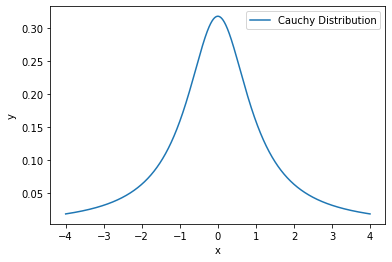
\includegraphics[width = 0.6\textwidth]{q3a.png}
  \caption{Cauchy(0,1) distribution}
\end{figure}
\noindent \textcolor{blue}{From here, we repeat this process for $B = 1000$ times and create a list containing all the sample means. Then, we plot a histogram of all the sample means, and superimpose a Standard Cauchy distribution over it. The histogram of means also follows a Cauchy(0,1) distribution. This is illustrated in the plot below. The code for generating this plot is also attached with the assignment.}
\begin{figure}[H]
  \centering
  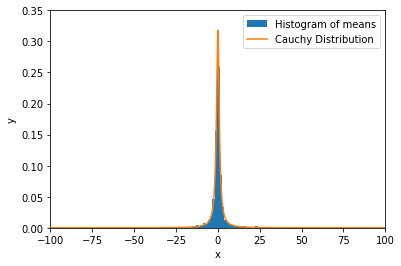
\includegraphics[width = 0.6\textwidth]{q3.png}
  \caption{Cauchy(0,1) distribution superimposed over Histogram of means}
\end{figure}
\noindent Now, for the second part of the problem, we can use the Likelihood function to estimate $\theta$. Since there is no closed form solution, we turn to numerical approximation methods implemented in Python. These methods are iterative, and convergence is acheived after set number of iterations. The methods are as follows
\begin{enumerate}[a.]
  \item Step-wise gradient ascent: Here, we have $\gamma^{m}$ as the learning rate.
  \begin{equation}
    \nonumber
    \theta^{m+1} = \theta^{m} + \gamma^{m}\frac{\partial \mathcal{L}(\theta^{m})}{\partial \theta}
  \end{equation}
  \item Newton-Raphson: Similar to gradient ascent, except our learning rate is computed as a function of the inverse of second gradient of the log likelihood function.
  \begin{equation}
    \nonumber
    \theta^{m+1} = \theta^{m} + J(\theta^{m})^{-1}\frac{\partial \mathcal{L}(\theta^{m})}{\partial \theta}
  \end{equation}
  \item stochastic gradient ascent.
  Here, we take a batch of values from our sample, and compute the gradients accordingly. Taking random batches from sample for each iteration helps us avoid saddle points, and helps us achieve convergence quickly.
  \begin{equation}
    \nonumber
    \theta^{m+1} = \theta^{m} + \gamma^{m}\frac{\partial \mathcal{L}_{i^{m}}(\theta^{m})}{\partial \theta}
  \end{equation}
\end{enumerate}
To estimate the first and the second gradient required in the implementations of these methods, we arrive at the following expression for the Log Likelihood function. We know that,
\begin{equation}
  \nonumber
  \begin{aligned}
    f(y_{i} | \theta, 1) & = \frac{1}{\pi} \frac{1}{1 + (y_{i} - \theta)^{2}}\\
    L(\theta) & =  \prod_{i = 1}^{n}\frac{1}{\pi} \frac{1}{1 + (y_{i} - \theta)^{2}}\\
    \mathcal{L}(\theta) & =  \sum_{i = 1}^{n} \text{log}\bigg(\frac{1}{\pi}\frac{1}{1 + (y_{i} - \theta)^{2}}\bigg)\\
    & = -\big[n\text{log}(\pi) + \sum_{i = 1}^{n} \text{log}(1 + (y_{i} - \theta)^{2}) \big]
  \end{aligned}
\end{equation}
Now, the first and second derivative can be calculated as,
\begin{equation}
  \nonumber
  \begin{aligned}
    \frac{\partial \mathcal{L}}{\partial \theta} & = -2 \sum_{i = 1}^{n}\frac{(y_{i} - \theta)}{1 + (y_{i} - \theta)^{2}}\\
    \frac{\partial^{2} \mathcal{L}}{\partial \theta^{2}} & = -2 \sum_{i = 1}^{n} \frac{[1 + (y_{i} - \theta)^{2}](-1) - (y_{i} - \theta)[2(y_{i} - \theta)]}{(1 + (y_{i} - \theta)^{2})^{2}}\\
    & = 2 \sum_{i = 1}^{n} \frac{1 + 3(y_{i} - \theta)^{2}}{(1 + (y_{i} - \theta)^{2})^{2}}
  \end{aligned}
\end{equation}
\textcolor{blue}{Using these derivate formulas, we can implement the methods given above. Our convergence criteria is met, when the total number of iterations reach 100000. For the stochastic gradient ascent, we consider a batch size of $12$. We also consider a learning rate of 0.5 for the stochastic and stepwise gradient ascent, and we consider an initial guess value for $\theta$ as 5 in all cases from where we iteratively try to find actual $\theta$. We arrive at the following results for the estimated values of $\theta$. We can verify the integrity of these results by fitting a cauchy distribution using the \emph{cauchy.fit()} method in \emph{scipy.stats}. Using this, we get a value for $\theta$ as $9.12286148071289$. Therefore, we can also calculate the rms error for each method as follows. The plots have also been attached.
\begin{enumerate}[a.]
  \item step-wise gradient ascent: $\theta = 7.637799268662628$, rms error: $1.485062212050262$
  \begin{figure}[H]
    \centering
    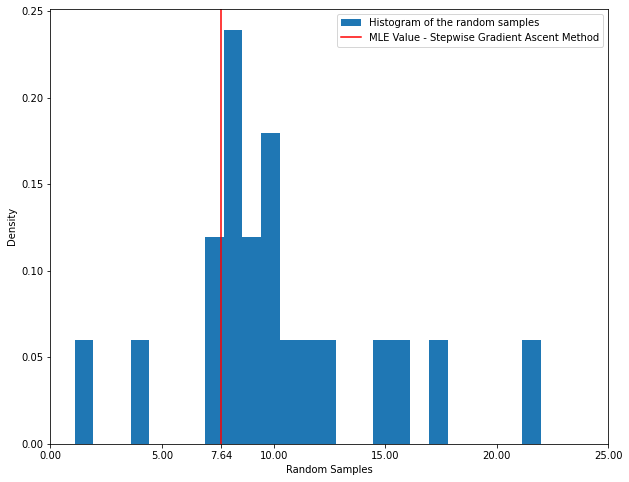
\includegraphics[width = 0.6\textwidth]{q3stepgrad.png}
    \caption{Stepwise Gradient Ascent method calculated theta}
  \end{figure}
  \item Newton-Raphson method: $\theta = 9.122853472425337$, rms error: $8.008287553096238 \times 10^{-6}$
  \begin{figure}[H]
    \centering
    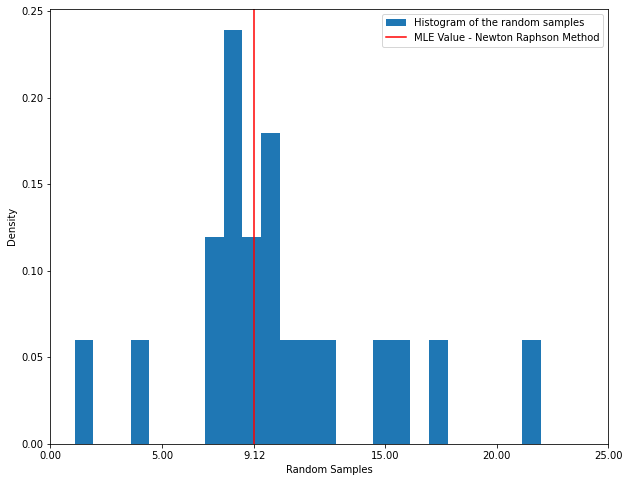
\includegraphics[width = 0.6\textwidth]{q3newtonraphson.png}
    \caption{Newton-Raphson method calculated theta}
  \end{figure}
  \item Stochastic gradient ascent: $\theta = 9.472881177927484$, rms error: $0.35001969721459325$
  \begin{figure}[H]
    \centering
    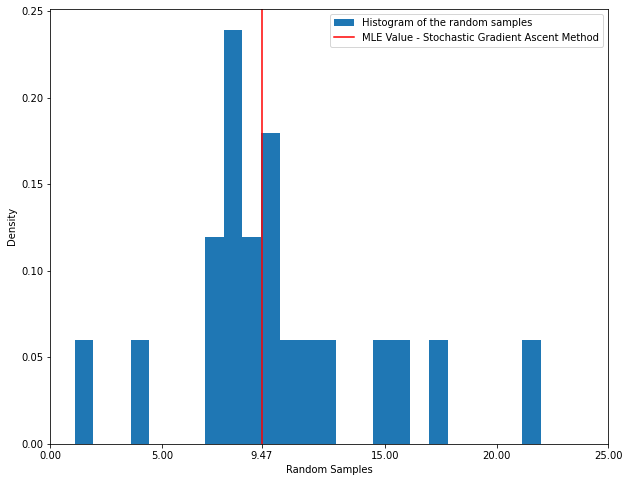
\includegraphics[width = 0.6\textwidth]{q3stocgrad.png}
    \caption{Stochastic gradient ascent method calculated theta}
  \end{figure}
\end{enumerate}
The code accomanying these implementations is attached along with this assignment.} \\ \\
\noindent \emph{4. Let $y_{ij} \overset{ind}{\sim} \text{Normal}(\mu_{i}, \sigma^{2})$, $i = 1 \dots n$ and $j = 1 \dots m$ with $n \rightarrow \infty$ but m fixed. Find out MLEs of $\mu_{i}$ and  $\sigma^{2}$. Show that $\hat{\sigma}_{MLE}^{2}$ is inconsistent for $\sigma^{2}$. Adjust this estimator to come up with a consistent estimator of $\sigma^{2}$.}\\ \\
\textbf{Solution:} It is given that
\begin{equation}
  \nonumber
  f(y_{ij} | \mu_{i}, \sigma^{2}) = \frac{1}{\sqrt{2\pi}\sigma}e^{\frac{-1}{2\sigma^{2}} (y_{i} - \mu_{i})^{2}}; \forall j = 1, \dots, m
\end{equation}
Now, the likelihood and the log likelihood function can be calculated as,
\begin{equation}
  \nonumber
  \begin{aligned}
    L(y_{ij} | \mu_{i}, \sigma^{2}) & = \prod_{i = 1}^{n} \frac{1}{\sqrt{2\pi}\sigma}e^{\frac{-1}{2\sigma^{2}} (y_{i} - \mu_{i})^{2}}; \forall j = 1 \dots m\\
    \mathcal{L}(y_{ij} | \mu_{i}, \sigma^{2}) & = \sum_{i = 1}^{n} \text{log}\bigg(\frac{1}{\sqrt{2\pi}\sigma}e^{\frac{-1}{2\sigma^{2}} (y_{i} - \mu_{i})^{2}}\bigg); \forall j = 1 \dots m\\
    & = \sum_{i = 1}^{n} \text{log}\bigg(\frac{1}{\sqrt{2 \pi} \sigma}\bigg) + \sum_{i = 1}^{n} \text{log} e^{\frac{-1}{2 \sigma^{2}} (y_{i} - \mu_{i})^{2}}\\
    & = -n\text{log}(\sqrt{2 \pi} \sigma) + \sum_{i = 1}^{n} \frac{-1}{2 \sigma^{2}}(y_{i} - \mu_{i})^{2}\\
  \end{aligned}
\end{equation}
Now, taking the derivative of the log likelihood function with respect to $\mu_{i}$ and $\sigma$, and solving them, we get the following results.
\begin{equation}
  \nonumber
  \begin{aligned}
    \frac{\partial \mathcal{L}}{\partial \sigma} & = -\frac{n}{\sigma} + \frac{1}{\sigma^{3}}\sum_{i = 1}^{n}(y_{i} - \mu_{i})^{2} = 0\\
    & = -n \sigma^{2} + \sum_{i = 1}^{n} (y_{i} - \mu_{i})^{2} = 0\\
    \hat{\sigma}_{MLE}^{2} & = \frac{1}{n}\sum_{i = 1}^{n}(y_{i} - \mu_{i})^{2}
  \end{aligned}
\end{equation}
\begin{equation}
  \nonumber
  \begin{aligned}
    \frac{\partial \mathcal{L}}{\partial \mu_{i}} & = 0 + \frac{1}{2 \sigma^{2}} \sum_{i = 1}^{n}(2)(y_{i} - \mu_{i}) = 0\\
    \hat{\mu}_{i,MLE} & = y_{i}
  \end{aligned}
\end{equation}
Therefore, we have found the MLEs for $\mu_{i}$ and  $\sigma^{2}$\\ \\
\noindent \emph{5. For $y_{1}, \dots, y_{n} \overset{iid}{\sim} \text{Uniform}(0, \theta)$, show that $z_{n} = \frac{n(\theta -  \hat{\theta}_{MLE})}{\theta} \xrightarrow{D} E$, where $E$ is exponential. Design a simulation study illustrating this nice result.}\\ \\
\textbf{Solution:} The given distribution is Uniform(0, $\theta$), and the pdf is given by
\begin{equation}
  \nonumber
  f(y_{i} | \theta) = \frac{1}{\theta}
\end{equation}
Let us construct the likelihood and log likelihood function for this distribution.
\begin{equation}
  \nonumber
  \begin{aligned}
    L(\theta) & = \prod_{i = 1}^{n} \bigg(\frac{1}{\theta}\bigg)\\
    & = \bigg(\frac{1}{\theta}\bigg)^{n}\\
    \mathcal{L}(\theta) & = -n\text{log}(\theta)
  \end{aligned}
\end{equation}
Therefore, since the function is monotonous, the MLE for $\theta$ is given by $y_{(n)}$, which is the nth order statistic. In simple words,
$\hat{\theta}_{MLE} = \text{max}\{y_{1}, \dots, y_{n}\}$. Now, we consider the given problem, $z_{n} = \frac{n(\theta -  \hat{\theta}_{MLE})}{\theta}$. The convergence in distribution is defined as when
\begin{equation}
  \nonumber
  \underset{n \rightarrow \infty}{\text{Lim}}\text{Pr}(x_{n} \leq a) = \text{Pr}(x \leq a)
\end{equation}
In our problem, as $n \rightarrow \infty$,
\begin{equation}
  \nonumber
  \begin{aligned}
    Pr(z_{n} \leq t) & = Pr\bigg(\frac{n(\theta - \hat{\theta}_{MLE})}{\theta} \leq t\bigg)\\
    & = Pr\bigg(n(\theta - \hat{\theta}_{MLE}) \leq \theta t\bigg)\\
    & = Pr\bigg(\hat{\theta}_{MLE} \geq \theta - \frac{\theta t}{n}\bigg)\\
    & = 1 - Pr\bigg(\hat{\theta}_{MLE} \leq \theta - \frac{\theta t}{n}\bigg)\\
    & = 1 - \bigg(\frac{\theta - \frac{\theta t}{n}}{\theta}\bigg)^{n}\\
    & = 1 - e^{-t}; \text{ Since } \underset{n \rightarrow \infty}{\text{Lim}} \bigg(1 + \frac{x}{n}\bigg)^{n} = e^{x}\\
  \end{aligned}
\end{equation}
This is the pdf of a exponential distribution with parameter $\lambda = 1$. Therefore we can conclude that for large n, $z_{n}$ converges in distribution to $E$. This is also illustrated in the graph below. The procudure to obtain the graph is also illustrated. We create a sorted array of a randomly generated uniform distribution with $\theta = 10$. For $B = 100000$ times, we generate random samples of size = 1000 from this population. The MLE of this sample is the maximum value of the samples, i.e., $\hat{\theta}_{MLE} = max\{x_{1}, x_{2} \dots, x_{n}\} = x_{(n)}$, as established above. By calculating the value of $z_n$ as asked in the question, and by taking the plot of $z_n$ overlaid with an exponential, we can see that the distribution converges. The code for generating this plot is also attached along with this assignment.
\begin{figure}[H]
  \centering
  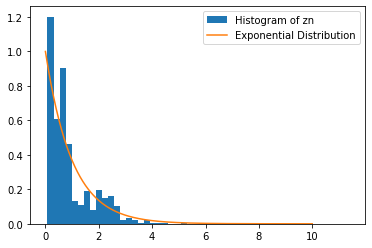
\includegraphics[width = 0.6\textwidth]{q5.png}
  \caption{Showing convergence in distribution}
\end{figure}
\noindent 6. Consider the spring failure data from Davison, providing the failure
times at stress 950 $\text{N}/\text{mm}^{2}$ in $10^{3}$ cycles:
\begin{center}
  $225, 171, 198, 189, 189, 135, 162, 135, 117, 162$
\end{center}
Using the method of maximum likelihood, fit a Weibull distribution to these data
[use the parametrization considered in class]. Also find an approximate 90\% joint
confidence region for the parameters $(k, \lambda)$. Supplement your analysis with appropriate plots.\\ \\
\textbf{Solution:}
The pdf of a Weibull distribution is given by
\begin{equation}
  \nonumber
  f(y_{i} | k, \lambda) = \frac{k}{\lambda}\bigg(\frac{y_{i}}{\lambda}\bigg)^{k - 1}e^{-(\frac{y_{i}}{\lambda})^{k}}
\end{equation}
We can find the likelihood and log likelihood function as follows.
\begin{equation}
  \nonumber
  \begin{aligned}
    L(\theta) & = \prod_{i = 1}^{n} \frac{k}{\lambda}\bigg(\frac{y_{i}}{\lambda}\bigg)^{k - 1}e^{-(\frac{y_{i}}{\lambda})^{k}}\\
    \mathcal{L}(\theta) & = \sum_{i = 1}^{n} \text{log}\bigg(\frac{k}{\lambda}\bigg(\frac{y_{i}}{\lambda}\bigg)^{k - 1}e^{-(\frac{y_{i}}{\lambda})^{k}}\bigg)\\
    & = n \text{log}(k) - nk \text{log}(\lambda) - \sum_{i = 1}^{n} \bigg(\frac{y_{i}}{\lambda}\bigg)^{k} + (k - 1)\sum_{i = 1}^{n} \text{log}(y_{i})
  \end{aligned}
\end{equation}
Taking the partial derivate wrt. $k, \lambda$, and equating to zero, we get
\begin{equation}
  \nonumber
  \begin{aligned}
      \frac{\partial \mathcal{L}}{\partial \lambda} & = -\frac{nk}{\lambda} + \frac{k}{\lambda^{k + 1}} + \frac{k}{\lambda^{k + 1}} \sum_{i = 1}^{n} (y_{i})^{k} & = 0\\
      \frac{\partial \mathcal{L}}{\partial k} & = \frac{n}{k} - n \text{log}(\lambda) - \frac{\sum_{i = 1}^{n}y_{i}^{k} - \text{log}(\lambda) \sum_{i = 1}^{n} y_{i}^{k}}{\lambda^{k}} & = 0
  \end{aligned}
\end{equation}
From the first equation, we can arrive at a value for $\hat{\lambda}$ as
\begin{equation}
  \nonumber
  \hat{\lambda} = \bigg(\sum_{i = 1}^{n} y_{i}^{k} \bigg)^{\frac{1}{k}}
\end{equation}
We cannot solve the second equation directly to find $\hat{k}$, therefore we use the Newton Raphson method to find an iterative solution for $\hat{k}$ in the second equation. We update $\hat{k}_{new}$ as
\begin{equation}
  \nonumber
  \begin{aligned}
    \hat{k}_{new} = \hat{k}_{old} - \frac{f(\hat{k}_{old})}{f'(\hat{k}_{old})}
  \end{aligned}
\end{equation}
The derivative can be calculated as
\begin{equation}
  \nonumber
  \frac{\partial^{2} \mathcal{L}}{\partial k^{2}} = \bigg(\frac{\sum_{i = 1}^{n}y_{i}^{k}\text{log}y_{i} }{\sum_{i = 1}^{n} y_{i}^{k}}\bigg)^{2} - 2\bigg(\frac{\sum_{i = 1}^{n}y_{i}^{k}\text{log}y_{i} }{\sum_{i = 1}^{n} y_{i}^{k}}\bigg) - \frac{1}{k^{2}}
\end{equation}
Our stopping criterion is reached, until the first derivative value hits 0.0001. This is also the point where the increment in $\hat{k}_{new}$ is negligible compared to $\hat{k}_{old}$. We use the value of $k_{new}$ in our original expression to estimate $\hat{\lambda}$. Using this procudure, for the given data, we get the following parameter values
\begin{equation}
  \nonumber
  (\hat{k}, \hat{\lambda}) = (5.974797076433545, 181.40553454869354)
\end{equation}
We can verify the integrity of these results by using the \emph{weibull\_min.fit()} function in the \emph{scipy.stats} package and estimating the parameters. The RMS value of the errors are
\begin{equation}
  \nonumber
  \begin{aligned}
    e_{k} & = (\hat{k} - k)^{2} = 0.00000447717\\
    e_{\lambda} & = (\hat{\lambda} - \lambda)^{2} = 1.15940309 \times 10^{-9}
  \end{aligned}
\end{equation}
Therefore, we can conclude that our estimates are pretty accurate and our method works. Now, using this estimated values of $(\hat{k}, \hat{\lambda})$, we can calculate the joint confidence region as follows. \\ \\
\noindent 7. For a Weibull($k, \lambda$) distribution, design a simulation study to show that $(\mathbf{\hat{\theta}} - \mathbf{\theta})^{T}(\mathbf{J}(\hat{\theta}))(\mathbf{\hat{\theta}} - \mathbf{\theta}) \xrightarrow{D} \chi^{2}_{2}$ and $\mathbf{W}(\theta) \xrightarrow{D} \chi^{2}_{2}$\\ \\
\textbf{Solution:}
The pdf of a Weibull distribution is given by
\begin{equation}
  \nonumber
  f(x_{i} | k, \lambda) = \frac{k}{\lambda}\bigg(\frac{x_{i}}{\lambda}\bigg)^{k - 1}e^{-(\frac{x_{i}}{\lambda})^{k}}
\end{equation}
For this question, let us consider the following.
\begin{equation}
  \nonumber
  \begin{aligned}
    \mathbf{\hat{\theta}} & = [\hat{k}, \hat{\lambda}]\\
    \mathbf{\theta} & = [k, \lambda]
  \end{aligned}
\end{equation}
The likelihood function is given by,
\begin{equation}
  \nonumber
  \mathcal{L}(\theta) = -kn\text{log}(\lambda) + n \text{log}(k) + (k - 1)\sum_{i = 1}^{n}\text{log}(x_{i}) - \sum_{i = 1}^{n}\bigg(\frac{x_{i}}{\lambda}\bigg)^{k}\\
\end{equation}
We find the first and second derivatives of this log-likelihood function as follows.
\begin{equation}
  \nonumber
  \begin{aligned}
    \frac{\partial \mathcal{L}(\theta)}{\partial k} & = -n \text{log}(\lambda) - \sum_{i = 1}^{n}\bigg(\frac{x_{i}}{\lambda}\bigg)^{k}\text{log}\bigg(\frac{x_{i}}{\lambda}\bigg) + \sum_{i = 1}^{n}\text{log}(x_{i}) + \frac{n}{k}\\
    \frac{\partial \mathcal{L}(\theta)}{\partial \lambda} & = \frac{-kn}{\lambda} +  \sum_{i = 1}^{n}\frac{k(\frac{x_{i}}{\lambda})^{k}}{\lambda}\\
    \frac{\partial^{2} \mathcal{L}(\theta)}{\partial k^{2}} & = \sum_{i = 1}^{n}\bigg(\frac{x_{i}}{\lambda}\bigg)^{k}\text{log}\bigg(\frac{x_{i}}{\lambda}\bigg)^{2} - \frac{n}{k^{2}}\\
    \frac{\partial^{2} \mathcal{L}(\theta)}{\partial \lambda^{2}} & = \frac{kn}{\lambda^{2}} - \sum_{i = 1}^{n}\bigg(\frac{k^2 (\frac{x_{i}}{\lambda})^{k}}{\lambda^{2}} + \frac{k(\frac{x_{i}}{\lambda})^{k}}{\lambda^{2}}\bigg)\\
    \frac{\partial^{2} \mathcal{L}(\theta)}{\partial \lambda \partial k} & = -\sum_{i = 1}^{n}\bigg(-\frac{k(\frac{x_{i}}{\lambda})^{k}\text{log}(\frac{x_{i}}{\lambda})}{\lambda} - \frac{(\frac{x_{i}}{\lambda})^{k}}{\lambda}\bigg) - \frac{n}{\lambda} = \frac{\partial^{2} \mathcal{L}(\theta)}{\partial k \partial \lambda }\\
  \end{aligned}
\end{equation}
Using the second derivate values, we can calculate $\mathbf{J}(\theta)$ as,
\begin{equation}
  \nonumber
  \begin{aligned}
    \mathbf{J}(\theta) & = \begin{bmatrix}
      -\frac{\partial^{2} \mathcal{L}(\theta)}{\partial k^{2}} & -\frac{\partial \mathcal{L}(\theta)}{\partial k \partial \lambda}\\
      -\frac{\partial \mathcal{L}(\theta)}{\partial \lambda \partial k } & -\frac{\partial^{2} \mathcal{L}(\theta)}{\partial \lambda^{2}}\\
  \end{bmatrix}\\
  \mathbf{J}(\hat{\theta}) & = \begin{bmatrix}
    -\frac{\partial^{2} \mathcal{L}(\theta)}{\partial k^{2}} \rvert_{\hat{k}, \hat{\lambda}} & -\frac{\partial \mathcal{L}(\theta)}{\partial k \partial \lambda} \rvert_{\hat{k}, \hat{\lambda}}\\
    -\frac{\partial \mathcal{L}(\theta)}{\partial \lambda \partial k }\rvert_{\hat{k}, \hat{\lambda}} & -\frac{\partial^{2} \mathcal{L}(\theta)}{\partial \lambda^{2}}\rvert_{\hat{k}, \hat{\lambda}}
  \end{bmatrix}
  \end{aligned}
\end{equation}
Also, we have the following vectors,
\begin{equation}
  \begin{aligned}
    \nonumber
    \begin{matrix}
      (\hat{\theta} - \theta)
    \end{matrix}^{T} & = \begin{bmatrix}
      \hat{k} - k &
      \hat{\lambda} -\lambda
    \end{bmatrix}
  \end{aligned}
\end{equation}
\begin{equation}
  \begin{aligned}
    \nonumber
    \begin{matrix}
      \hat{\theta} - \theta
    \end{matrix} & = \begin{bmatrix}
      \hat{k} - k \\
      \hat{\lambda} -\lambda
    \end{bmatrix}
  \end{aligned}
\end{equation}
By combining the expressions, we arrive at the following result.
\begin{equation}
  \nonumber
  \begin{aligned}
    (\hat{\theta} - \theta)^{T}\mathbf{J}(\hat{\theta})(\hat{\theta} - \theta) & = \begin{bmatrix}
      \hat{k} - k &
      \hat{\lambda} -\lambda
    \end{bmatrix}\begin{bmatrix}
      -\frac{\partial^{2} \mathcal{L}(\theta)}{\partial k^{2}} \rvert_{\hat{k}, \hat{\lambda}} & -\frac{\partial \mathcal{L}(\theta)}{\partial k \partial \lambda} \rvert_{\hat{k}, \hat{\lambda}}\\
      -\frac{\partial \mathcal{L}(\theta)}{\partial \lambda \partial k }\rvert_{\hat{k}, \hat{\lambda}} & -\frac{\partial^{2} \mathcal{L}(\theta)}{\partial \lambda^{2}}\rvert_{\hat{k}, \hat{\lambda}}
    \end{bmatrix}
    \begin{bmatrix}
      \hat{k} - k \\
      \hat{\lambda} -\lambda
    \end{bmatrix}\\
    & = \bigg[(- k + \hat{k}) ((- k + \hat{k}) \bigg(\sum_{i=1}^{n} \bigg(\frac{{x}_{i}}{\hat{\lambda}}\bigg)^{\hat{k}} \log{\bigg(\frac{{x}_{i}}{\hat{\lambda}}\bigg)}^{2} + \frac{n}{\hat{k}^{2}}\bigg) + \\
    & (\hat{\lambda} - \lambda) \bigg(\sum_{i=1}^{n}\bigg(- \frac{\hat{k} (\frac{{x}_{i}}{\hat{\lambda}})^{\hat{k}} \log{(\frac{{x}_{i}}{\hat{\lambda}} )}}{\hat{\lambda}} - \frac{(\frac{{x}_{i}}{\hat{\lambda}})^{\hat{k}}}{\hat{\lambda}}\bigg) + \frac{n}{\hat{\lambda}}\bigg)\bigg)\\
    & + (\hat{\lambda} - \lambda) ((- k + \hat{k}) \bigg(\sum_{i=1}^{n} \bigg(- \frac{\hat{k} (\frac{{x}_{i}}{\hat{\lambda}})^{\hat{k}} \log{(\frac{{x}_{i}}{\hat{\lambda}} )}}{\hat{\lambda}} - \frac{(\frac{{x}_{i}}{\hat{\lambda}})^{\hat{k}}}{\hat{\lambda}}\bigg) + \frac{n}{\hat{\lambda}}\bigg) +\\
    & (\hat{\lambda} - \lambda) \bigg(- \frac{\hat{k} n}{\hat{\lambda}^{2}} + \sum_{i=1}^{n} \bigg(\frac{\hat{k}^{2} (\frac{{x}_{i}}{\hat{\lambda}})^{\hat{k}}}{\hat{\lambda}^{2}} + \frac{\hat{k} (\frac{{x}_{i}}{\hat{\lambda}})^{\hat{k}}}{\hat{\lambda}^{2}}\bigg)\bigg)\bigg)\bigg]
  \end{aligned}
\end{equation}
We have to show that this expression $\xrightarrow{D} \chi_{2}^{2}$. Similarly, we can get the expression for $\mathbf{W}(\theta)$. It is given by,
\begin{equation}
  \nonumber
  \mathbf{W}(\theta) = 2\text{log}\bigg\{\frac{L(\hat{\theta}_{MLE})}{L(\theta)}\bigg\} = 2\bigg\{\mathcal{L}({\hat{\theta}_{MLE}}) - \mathcal{L}({\theta})\bigg\}
\end{equation}
We also get an expression for this $\mathbf{W}(\theta)$ and show that $\mathbf{W}(\theta) \xrightarrow{D} \chi_{2}^{2}$
\end{document}
